In this chapter I present preliminary surface stress and adhesion energy data collected for two types of silicone with various stiffnesses. We first used Gelest to obtain our preliminary data and tune the operation of our device. We then switched to Dow-Corning to continue more extensive measurements. First we give a brief background of the materials used. 


\section{Organosilicon Polymer Chemistry}
\label{section:polychem}
PDMS, or Poly-Dimethyl-Siloxane, is a commonly used polymer gel in the field of soft condensed matter. The gel is composed of a polymer network connected by crosslinkers, with additional free polymer in the fluid phase. When stretched, the the large number of covalent bonds resist deformation on a macroscopic level.\footnote{PDMS consists of covalent crosslinkers, though many compliant materials are a result of physical crosslinkers (e.g. gelatin). When physical crosslinkers are stretched,the configuration of the system changes such that the tangled crosslinkers begin to unwind and untangle. From a statistical mechanics perspective, this decreases the configurational entropy, thus increasing the free energy.} 

%physical crosslinkers: add to ch1 brief descriptions.
%When stretched, the configuration of the system changes such that the tangled crosslinkers begin to unwind and untangle. From a statistical mechanics perspective, this decreases the configurational entropy, thus increasing the free energy. 

Below (Fig. \ref{fig:DMS-V31}) is the chemical structure for the vinyl-terminated PDMS (Gelest) that comprises the fluid phase. 
% Set chemical bonds length
\setatomsep{20pt}

% -------------From chemfig manual, useful macro--------------------
\newcommand\setpolymerdelim[2]{\def\delimleft{#1}\def\delimright{#2}}
\def\makebraces(#1,#2)#3#4#5{%
	\edef\delimhalfdim{\the\dimexpr(#1+#2)/2}%
	\edef\delimvshift{\the\dimexpr(#1-#2)/2}%
	\chemmove{
		\node[at=(#4),yshift=(\delimvshift)]
		{$
			\left\delimleft
			\vrule height\delimhalfdim depth\delimhalfdim width0pt
			\right.
			$};
		\node[at=(#5),yshift=(\delimvshift)]
		{$
			\left.
			\vrule height\delimhalfdim depth\delimhalfdim width0pt
			\right\delimright_{\rlap{#3}}
			$};
	}%
}

%PDMS DMS-V31 Figure
\begin{figure}[h!]
	\centering
	\scalebox{1.75}{
		\setpolymerdelim()
		
		\chemfig{H_2C=C(-[-3]H)--[@{op,0}]Si(-[2]CH_3)(-[6]CH_3)-O--[@{cl,0}]Si(-[2]CH_3)(-[6]CH_3)-C(-[7]H)=CH_2}
		
		\makebraces(20pt,20pt){$\!\!n$}{op}{cl}
	}
	\label{fig:DMS-V31}
	\caption[DMS-V31]{Divinyl-terminated Polydimethylsiloxane (DMS-V31)}
\end{figure}

The crosslinker for the system is a trimethylsiloxane terminated 25-35\% methylhydrosiloxane - dimethylsiloxane copolymer. The crosslinker is much shorter on average than the PDMS, containing roughly 20-30 repeating monomer groups. The single hydrogen on the methylhudrosiloxane is weakly bound, and can be replaced by one of the hydrogen atoms in the PDMS. This bonding happens over and over again, creating the long twisted chains that create the mesh network of the gel. Increasing density of crosslinkers provides an easy and controllable method to vary the gel's stiffness \cite{Andreotti2020}.

%PDMS Crosslinker HMS-301 Figure
\begin{figure}
	\centering
	\scalebox{1.75}{
		\setpolymerdelim()
		%the [@{op,offset}] and [@{cl,offset}] are for the giant parentheses macro function.
		\chemfig{H_3C-Si(-[2]CH_3)(-[6]CH_3)-O--[@{op,0}]Si(-[2]H)(-[6]CH_3)-O-[@{cl,.5}]-[@{op2,.5}]Si(-[2]CH_3)(-[6]CH3)-O--[@{cl2,0}]Si(-[2]CH_3)(-[6]CH_3)-CH_3}
		
		\makebraces(20pt,20pt){$\!\!m$}{op}{cl}
		\makebraces(20pt,20pt){$\!\!n$}{op2}{cl2}
	}		
	\label{fig:HMS-301}
	\caption[HMS-301]{Trimethylsiloxane terminated 25-35\% methylhydrosiloxane ($m$) - dimethylsiloxane ($n$). This is the crosslinker.}
\end{figure}

\begin{table}[h!]
	\begin{center}
		\begin{tabular}{|c||c||c|}
			\hline
			Mix Ratio (A:B) & Young's Modulus (kPa) & Sol Fraction (\%)\\
			\hline
			$7.5:1$ & $2.5 \,\pm\, 0.1$ & 65.2\\
			\hline
			$9:1$ & $5.0 \, \pm\, 0.1$  & 64.7\\
			\hline
			$11:1$ & $10.0 \,\pm\, 1$  & 63.7\\
			\hline
		\end{tabular}
	\end{center}
	\label{tab:recipes}
	\caption[PDMS ratios Characterization]{PDMS gel characterization for Gelest DMS-V31. By varying the relative density of the crosslinkers, one can predictably control the stiffness of the gel.}
\end{table}




\subsubsection{Silicone Preparation and Spin Coating}\todo[inline,color=pink]{Need to make sure this isn't too repetive for the ch2 section.}
Before spin-coating it is useful to coat the underlayer with fluorescent beads. It is not vital, but this is helpful in determining the substrate's thickness. The only information obtained by this coating is the location of the substrate's bottom surface, so a dense bead coverage is not required, and could potentially be harmful if there is light bleeding. We coat the bottom surface with 40nm beads for 30seconds - 1 minute. Full directions for preparing a fluroescent bead solution can be found in Appendix B. After this time, we return the fluorescent beads back to the solution for re-use. A significant number of beads will remain on the underlayer, however. To remove some excess, we gently wash the substrate with de-ionized water. For a coverslip, simply submerge the entire slip in water and gently remove it at a 45\degree angle, trying to prevent the water from breaking-up into smaller droplets. This process is slightly more difficult for the petri dish due to the larger size. We have had success using a very large container of water (large opening, not depth). Generally, we have used a 1000mL beaker tilted at an angle. It is also possible to use an autopipet for washing - simply repeat the same process used for the fluorescent bead coating, only use water this time. I have had mixed success with this technique, however, as it leaves a water droplet and often creates an uneven coating of fluorescent beads, manifested as streaks across the surface.

After the first layer of fluorescent beads is coated, it is time to spin coat the soft substrate. We aim to make our spin-coated substrates around 100 $\mu m$. Generally, our are between $80-100$ $\mu m$. Depending on the silicone, a different amount of time should be waited before spin coating onto the desired surface. We coat our substrate onto glass for "zero applied strain" data or onto PDMS \emph{yeah I gotta look up the brand when I get back. I totally forget.} for stretching data. It is best that the silicone is far enough along in the curing process that it has enough stiffness and cohesiveness to remain on the underlayer when spun. As an extreme example, consider trying to spin-coat water; it would all fling off the underlayer. \emph{is there a better term than underlayer. I'm thinking of the general term for what we use a coverslip or stretchy circle}. For Gelest 9:1, there is no waiting time necessary; Gelest 9:1 cures rapidly. For Dow Corning 1:1, a wait time before spinning of 1 hour was observed. 


To help with the evenness of the coating, we degas the gel by leaving it in a vacuum chamber for a few minutes. A few small bubbles are not of concern, as the process of transferring the gel to the underlayer is enough to pop any remaining stragglers. We have found that a "glob" of gel roughly half the diameter of the underlayer, with the spin-coater set to 500rpm for 40sec, is enough to create an even coating of roughly 100 $\mu m$ for both Gelest 9:1 and Dow-Corning 1:1 PDMS.

Coating a coverslip with silicone is a straightfoward process where hardly anything can go wrong. Coating the stretchable PDMS underlayer, however, requires some creativity to find the steps necessary to return the best results. I cut the PDMS disk with an X-acto knife and using a standard Petri\todo[color=pink]{ ...double check} dish (2.5in diameter) as a template. In order to avoid snagging, we cut out the circle before removing the paper sheets on both sides of the silicone. Taping the Petri dish to the paper is also helpful prevent the dish from slipping while cutting. Unlike the glass coverslip, the PDMS underlayer is not rigid and must be place on a ridgid surface, such as a Petri dish, for spin coating. This leaves the possibility for air bubbles to become trapped in between the PDMS and the Petri dish. This is a surefire way to ensure an unevenly coated substrate. To avoid this, we remove the top paper sheet of the newly cut PDMS, then place the Petri dish down upon the exposed silicone. This creates dish with a silicone disk on top and a paper sheet on top of that. We then push all the air bubbles out from the center outwards with out thumbs. Finally, any tiny air bubbles can hopefully be removed by placing the Petri dish in a vacuum chamber for a few minutes. It is at this point that we coat the PDMS with fluorescent beads and wash as desired before placing the petri dish onto the spin-coater and proceeding as described above.

After spin-coating, the silicone requires time to cure. We cure Dow-Corning 1:1 for at room temperature for at least 24 hours. For Gelest 9:1, we oven cure at $70 \degree$ C for at least 24 hours. Either silicone can be cured at room temperature or in the oven so long as a sufficient amount of time is waited, however, we have used this methods to maintain consistency, as well as parallel the techniques used in previous literature \cite{xu2017direct}.

After the silicone cures, we coat the surface with fluorescent beads again. It is important that the beads are dense enough to give a high resolution, yet not so dense as to become indistinguishable. For the 40nm bead solution prescribed in Appendix B, we allow the solution to soak for up to 1.5 minutes before removing and washing the substrate. While the fluorescent beads chosen are most susceptible to light at 440 nm, there is still the risk of photo-bleaching the fluorophores, and it is worth dimming the lights in the lab when working with them. 

\section{Preliminary Data: Gelest}
Because Figure \ref{fig:2017natcomfig} was obtained using Dow-Corning silicone gel, our intention from the start was to use this material in our adhesion based measurements. Because the material was back-ordered, we used Gelest instead while we calibrated the process. I present this preliminary data because it shows clear incremental steps of evidence that the surface stress for the substrate is increasing under strain.  

\subsection{Standard Candles}
Not only do we measure the depth and radii for a range of spheres, but we also measure a select few spheres at every strain. This allows us to track how any given sphere is changing, increasing our confidence that the shift in $\Upsilon$ and W is not just an artifact of noise. Below is the side profile for Gelest 9:1 ($\text{E}=6.3$ kPa). Notice how the profile shifts noticeably upwards to be flattened when the substrate is stretched. This shift is expected if the surface stress is increasing (see equation \ref{THEeqn}).

\begin{figure}[h!]
	\centering
	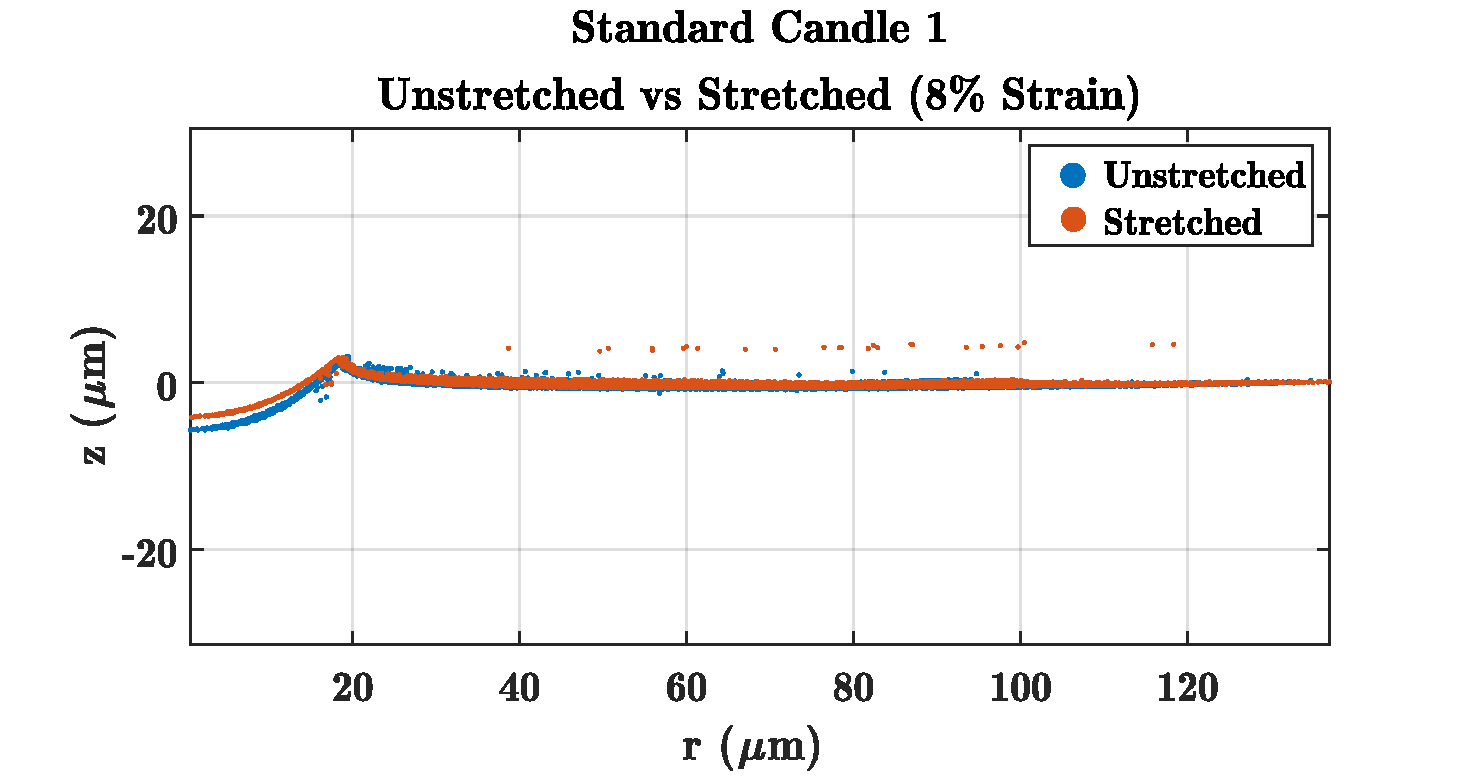
\includegraphics[width=\linewidth]{Chapters/Figures/sc1_unstretched_v_8ml}
	\caption[Side Collapse Comparison]{The side profile of the same sphere before and after stretch. Notice how after stretching, the sphere's indentation into the substrate is shallower. Substrate is Gelest 9:1 ($\text{E}=6.3$ kPa).}	
	\label{fig:sc1unstretchedv8ml}
\end{figure}

There is a lot of noise for D vs. R data collected with substrates on our stretching apparatus have a lot of noise. As seen in figure \ref{fig:glassvsstretched190218}, the D vs. R data collected on glass is far cleaner than that collected on the stretcher when strained. We can see the trend that under strain, the spheres sink into the substrate less deep. At 22\% strain, we expect zero strain-stiffening of our elastic substrate, and conclude that this change in depth is a result of an increase of surface stress, $ \Upsilon $. Unfortunately, the d vs. R values are too noisy/scattered to make a reasonable fit to extract $ W $ and $ \Upsilon $ values.

\begin{figure}[h!]
	\centering
	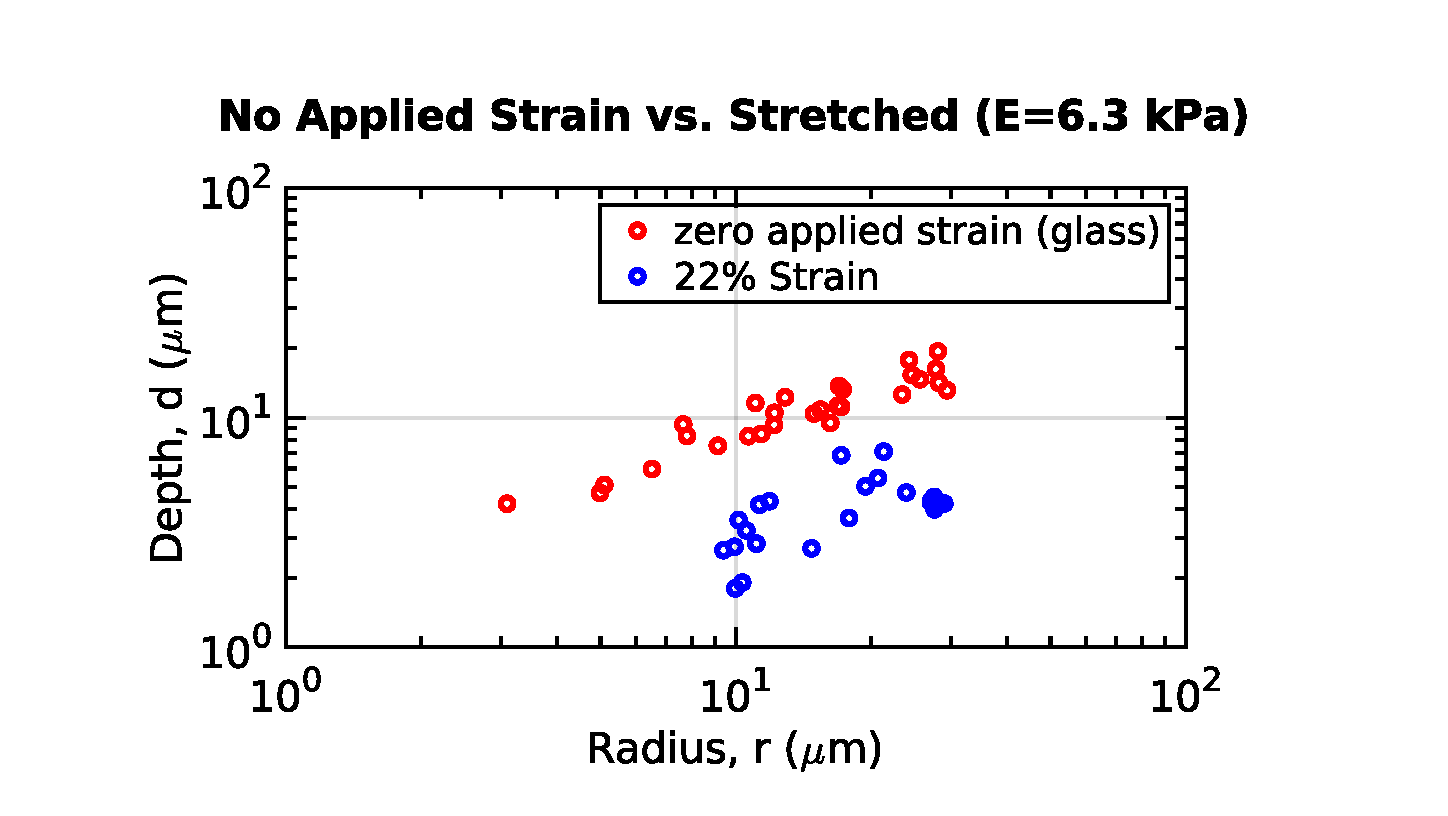
\includegraphics[width=\linewidth]{Chapters/Figures/glass_vs_stretched_190218}
	\caption[Glass vs. Stretched d vs. R]{For Gelest 9:1, the silicone under strain (blue) on average sinks less deep into the silicone than for the same silicone spun on glass (zero applied strain). The large noise for the strain-data meant we could not meaningfully determine $ \Upsilon $ and $ W $ to measure the variation in $ \Upsilon(\epsilon)$ and $W(\epsilon)$. \emph{COME BACK TO THIS AND FIX THE PLOT TO MAKE IT MATCH THE OTHERS}}
	\label{fig:glassvsstretched190218}
\end{figure}

\begin{figure}[h!]
	\centering
	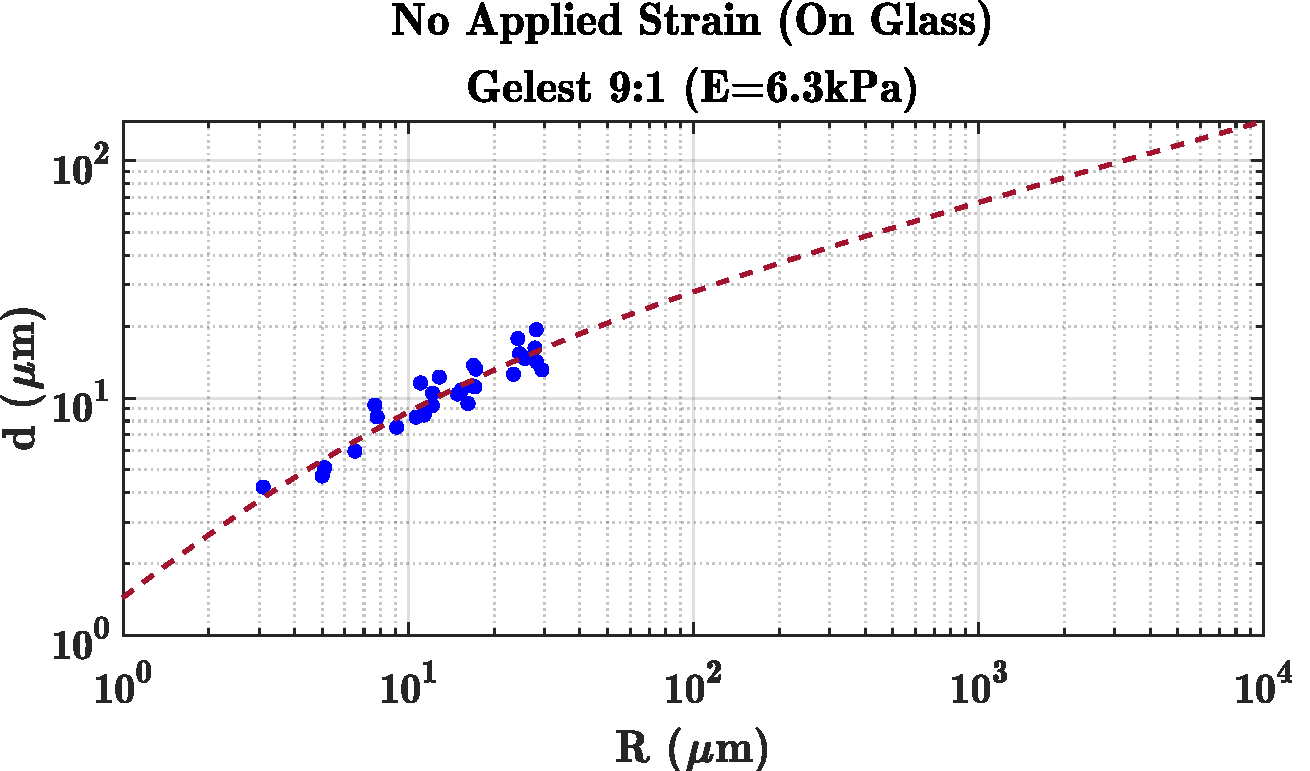
\includegraphics[width=\linewidth]{Chapters/Figures/w_ups_fit_G9-1}
	\caption[Gelest W-$\Upsilon$ Fit]{We fit Equation \ref{THEeqn} to the d vs. R plot for a Gelest 9:1 sample. The best fit line returns parameters of $ W=53 $  and $ \Upsilon=32 $ mNm$^{-1}$.}
	\label{fig:wupsfitg9-1}
\end{figure}

\section{Dow-Corning PDMS}
Because the $ \Upsilon(\epsilon) $ measurement in \textit{Nature Communications} 2017 \cite{xu2017direct} was conducted using a Dow-Corning PDMS substrate, we are especially interested in using this material for our $ \Upsilon(\epsilon) $ measurements. Because there has only been one measurement of $ \Upsilon(\epsilon) $ in soft matter, in order to have value to use as comparison, we need to use use the same material. 

Our first measurements with Dow-Corning PDMS returned largely varying results; the stiffness of the silicone varied by a factor of 2 from the expected value, and the stiffness continued to increase as the silicone cured over a period of several weeks, as opposed to the usual 24hr time-frame. Furthermore, the adhesion of the PDMS varied from sample to sample. Often the silica sphere would not adhere to the surface. It was eventually discovered that the Dow-Corning PDMS being used expired several years prior. Some of the measurements conducted, however, returned results of interest, and thus have been included here. 


\begin{figure}[h]
	\centering
	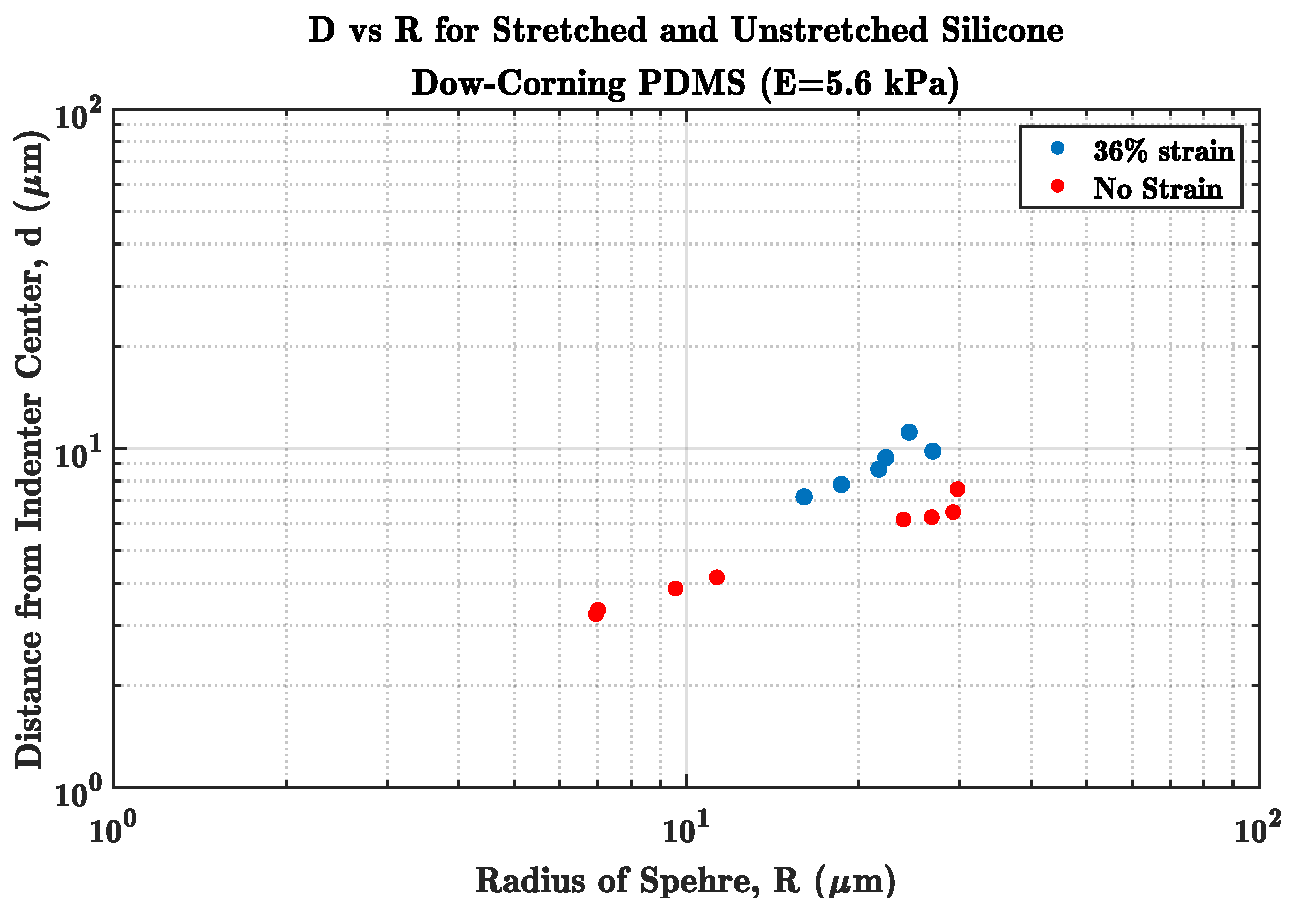
\includegraphics[width=\linewidth]{Chapters/Figures/d_vs_r_stretch_vs_no_stretch_DC181115}
	\caption[D vs. R Dow-Corning]{Here we plot D vs. R for a Dow-Corning PDMS Substrate at two different strains. Notice how at higher strains, the spheres sink in less deep. This can be explained by an increase in $\Upsilon$ or an increase in $E$ for the substrate.}
	\label{fig:dvsrstretchvsnostretchdc181115}
\end{figure}

\begin{figure}[h]
	\centering
	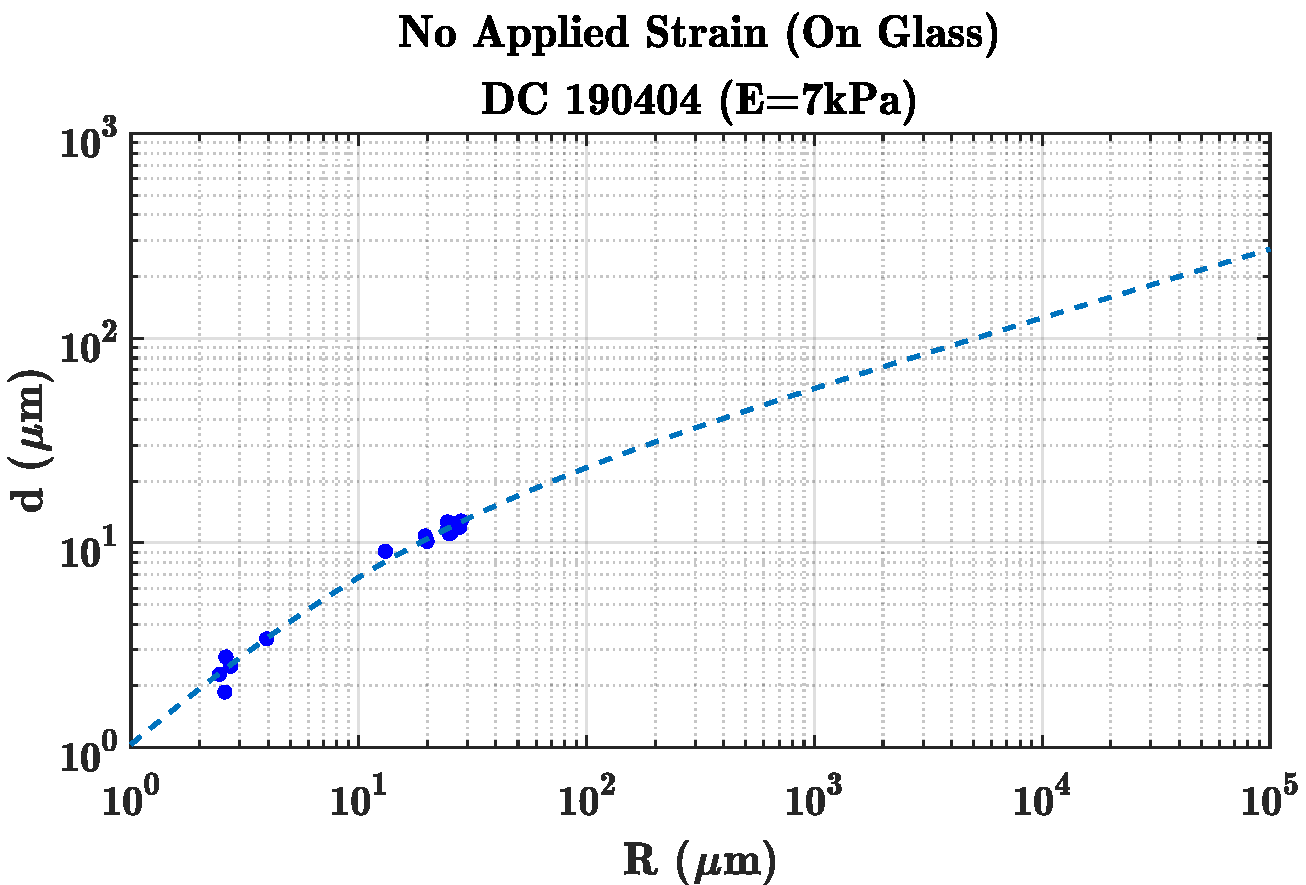
\includegraphics[width=\linewidth]{Chapters/Figures/WUps_fit_DC190404}
	\caption[Dow Corning W-$\Upsilon $ Fit]{The surface stress and adhesion energy fit for Dow Corning PDMS silicone with no applied strain. Given the d vs. R values, the fitting parameters to make the best fit line are W $ = 48.6$ and  $\Upsilon = 43.5$ mNm$^{-1}$.}
	\label{fig:wupsfitdc190404}
\end{figure}

\todo[inline,color=pink]{TexStudio broke the figures and writing up weirdly. Will fix later. Also, I have a stretchable Dow-corning substrate ready to go. I'd like to take this $ \Upsilon(\epsilon) $ measurement next week.}